\chapter{Tecnología}

\chapter{Capa de Tecnologia}

\section{Introducción}
En esta capa de aplicaciones observaremos los principales conceptos de comunicación entre componentes por medio de interfaces, donde en los siguientes diagramas se pueden observar los principales comportamientos del aplicativo mediante 4 puntos de vista: Comportamiento de aplicación, Cooperación de aplicación, Estructura de aplicación y el uso de la aplicación.\\
Tal como mencionamos anteriormente, en nuestra capa de aplicación se caracteriza por poseer una arquitectura de componentes, de tal forma que  mostramos las principales funciones dentro de cada componente y ademas como se relacionan y comunican cada uno de estos, de tal forma que observemos como sera el comportamiento y la logica de la aplicación

\section{Punto de Vista de Infraestructura}
\subsection{Descripción}


\subsubsection{Caso de Estudio}


\begin{figure}[H]
	\centering
	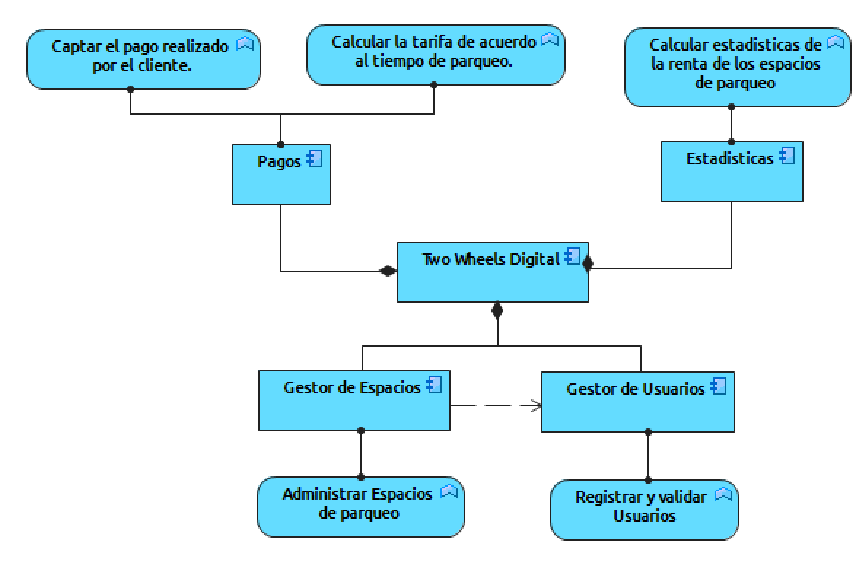
\includegraphics[width=1.0\textwidth]{imagenes/Caso_Estudio/Tecnologia/ComAplicacion.PDF}
	\caption{Caso de estudio: Punto de vista de Infraesructura.}
	\label{fig:gap_analysis}
\end{figure}

\section{Punto de Vista de Uso de Infraestructura}
\subsection{Descripción}


\subsubsection{Caso de Estudio}


\begin{figure}[H]
	\centering
	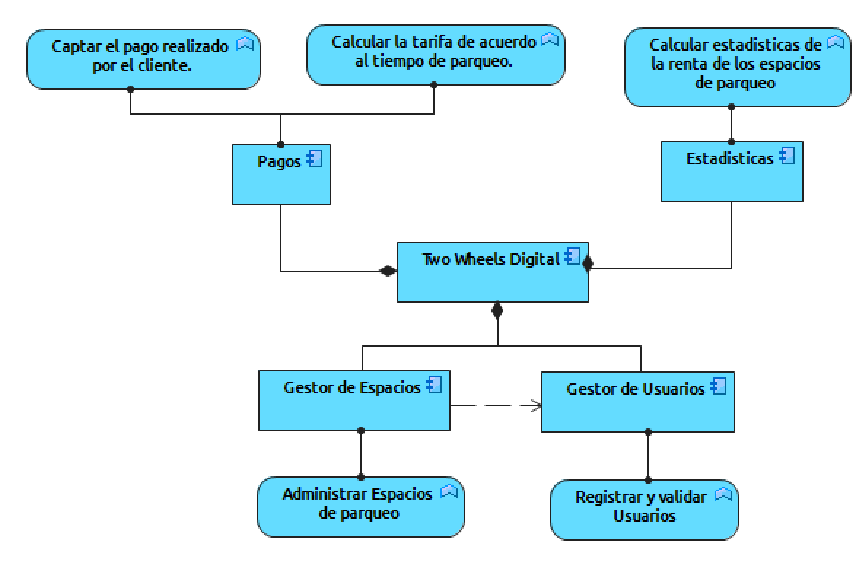
\includegraphics[width=1.0\textwidth]{imagenes/Caso_Estudio/Tecnologia/ComAplicacion.PDF}
	\caption{Caso de estudio: Punto de vista de Uso de Infraesructura.}
	\label{fig:gap_analysis}
\end{figure}


\section{Punto de Vista de Organización e implementación}
\subsection{Descripción}


\subsubsection{Caso de Estudio}


\begin{figure}[H]
	\centering
	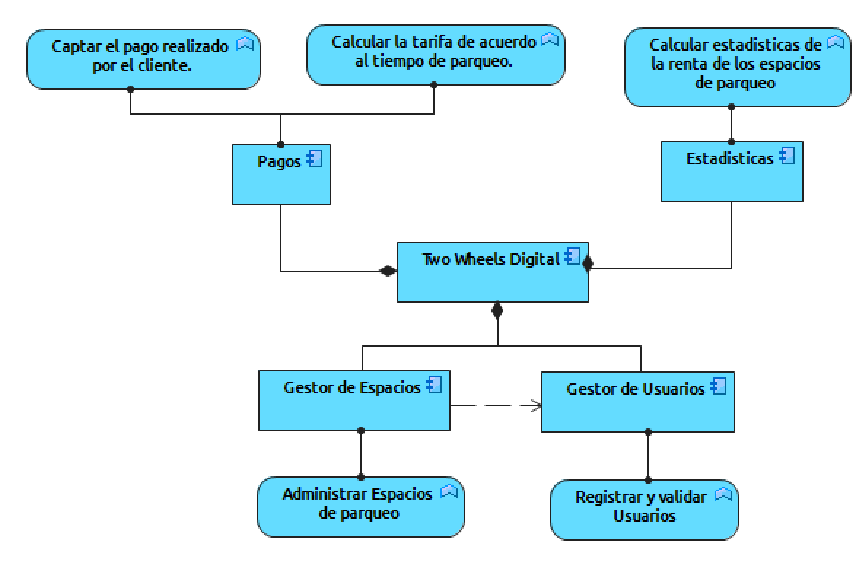
\includegraphics[width=1.0\textwidth]{imagenes/Caso_Estudio/Tecnologia/ComAplicacion.PDF}
	\caption{Caso de estudio: Punto de Vista de Organización e implementación.}
	\label{fig:gap_analysis}
\end{figure}


\section{Punto de Vista de Estructura de información}
\subsection{Descripción}


\subsubsection{Caso de Estudio}


\begin{figure}[H]
	\centering
	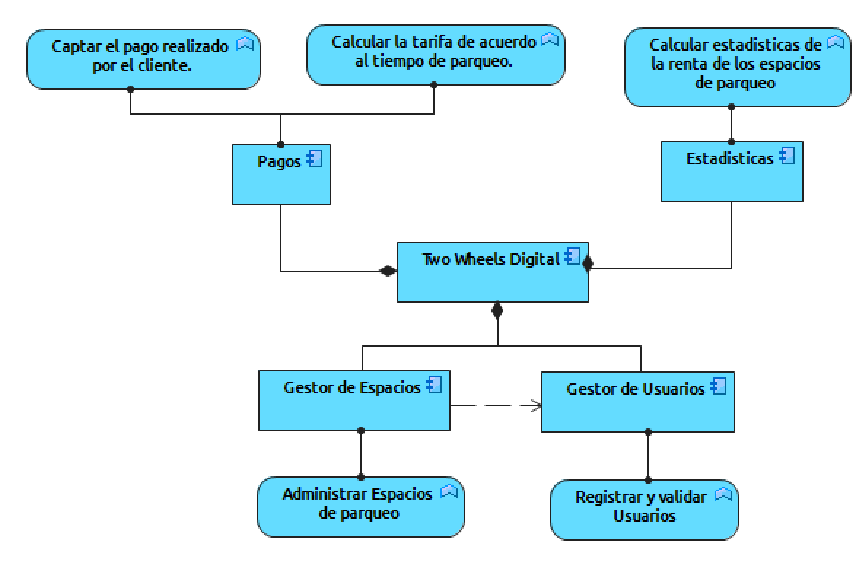
\includegraphics[width=1.0\textwidth]{imagenes/Caso_Estudio/Tecnologia/ComAplicacion.PDF}
	\caption{Caso de estudio: Punto de Vista de Estructura de información.}
	\label{fig:gap_analysis}
\end{figure}


\section{Punto de Vista de Realizacion del Servicio}
\subsection{Descripción}


\subsubsection{Caso de Estudio}

\begin{figure}[H]
	\centering
	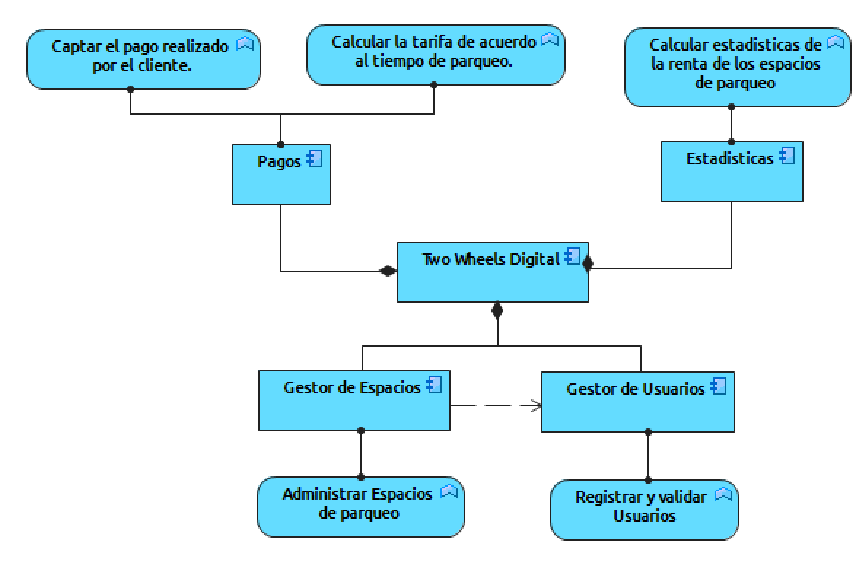
\includegraphics[width=1.0\textwidth]{imagenes/Caso_Estudio/Tecnologia/ComAplicacion.PDF}
	\caption{Caso de estudio: Punto de Vista de Realizacion del Servicio.}
	\label{fig:gap_analysis}
\end{figure}


\section{Punto de Vista de Capas}
\subsection{Descripción}


\subsubsection{Caso de Estudio}


\begin{figure}[H]
	\centering
	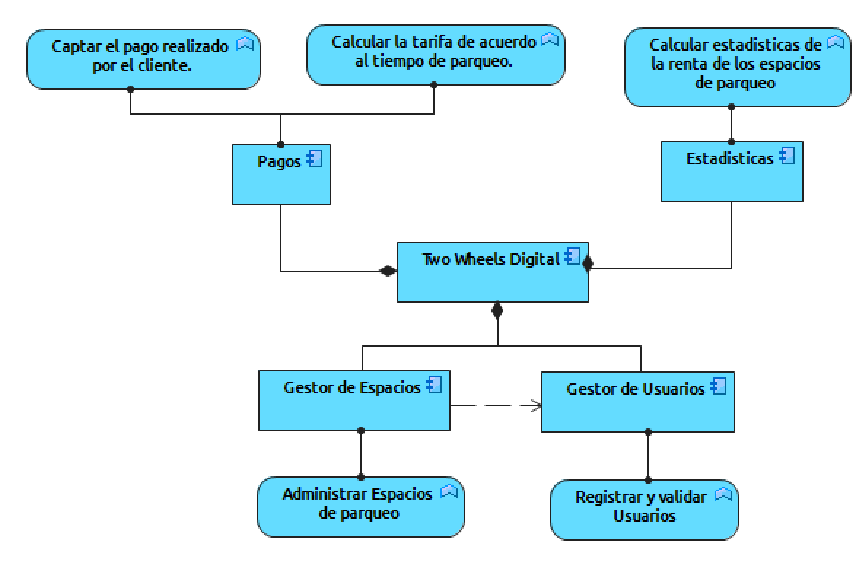
\includegraphics[width=1.0\textwidth]{imagenes/Caso_Estudio/Tecnologia/ComAplicacion.PDF}
	\caption{Caso de estudio: Punto de Vista de Capas.}
	\label{fig:gap_analysis}
\end{figure}

